% !TEX program = xelatex
% CUMCM 2026 A 题「药材的烘干问题」
% 编译器：XeLaTeX（ctex 需要）。TeX Live 2023+ / Overleaf 均可。
% 版式：A4、四边页边距 2.5 cm、匿名、无目录、从摘要页起页码从 1 连续编号。
\documentclass[a4paper,12pt]{ctexart}

\usepackage[a4paper,margin=2.5cm]{geometry}
\usepackage{amsmath,amssymb}
\usepackage{booktabs}
\usepackage{array}
\usepackage{graphicx}
\usepackage{float}
\usepackage{caption}
\usepackage[shortlabels]{enumitem}
\usepackage{siunitx}
\usepackage{xcolor}
\usepackage{tikz}
\usetikzlibrary{arrows.meta,positioning,calc,shapes.geometric,fit}
\usepackage{listings}

\sisetup{detect-all}
\graphicspath{{figures/}}
\captionsetup{font=small,labelsep=quad}
\setlength{\parskip}{3pt}
\linespread{1.25}

% ---- 统一记号 ----
\newcommand{\pd}[2]{\dfrac{\partial #1}{\partial #2}}
\newcommand{\Cbar}{\bar{C}}
\newcommand{\tstar}{t^{*}}
\newcommand{\tsamp}{t_{\mathrm{s}}}
\newcommand{\Cmax}{C_{\max}}
\newcommand{\Cenv}{C_{\mathrm{env}}}
\newcommand{\Tair}{T_{\mathrm{air}}}
\newcommand{\rhos}{\rho_{\mathrm{s}}}

% ---- 调色板（与插图一致）----
\definecolor{palBlueD}{HTML}{5271AE}
\definecolor{palBlueL}{HTML}{70ACDE}
\definecolor{palOrange}{HTML}{FFA660}
\definecolor{palGold}{HTML}{F5CC7D}
\definecolor{palRed}{HTML}{D85B59}

% ---- 源代码清单样式（附录）----
\lstset{
  basicstyle=\ttfamily\footnotesize,
  keywordstyle=\color{palBlueD}\bfseries,
  commentstyle=\color{gray!70!black}\itshape,
  stringstyle=\color{palRed},
  numbers=left, numberstyle=\tiny\color{gray}, numbersep=6pt,
  frame=single, rulecolor=\color{gray!40},
  breaklines=true, breakatwhitespace=false,
  columns=fullflexible, keepspaces=true, showstringspaces=false,
  extendedchars=true, tabsize=4, language=Python,
  aboveskip=6pt, belowskip=6pt,
}

\title{\vspace{-1.0cm}\textbf{药材热风干燥的径向传热传质模型与达标时长分析}}
\author{}
\date{}

\begin{document}
\maketitle
\thispagestyle{plain}

\begin{center}\textbf{摘\quad 要}\end{center}

药材热风干燥中，热量与水分在物料内部同时输运并受烘房环境驱动。本文以一根细长圆柱状药材为对象，忽略两端影响，沿半径方向建立\textbf{一维径向有效扩散--导热耦合模型}，统一求解题目的四个问题，给出温度场、含水率场与达标所需时间，并对结果作物理解释与可靠性检验。由于长直径比约为六比一，热量与水分主要沿半径进出，一维径向近似是合理的；模型清楚区分题给条件与建模假设，分别处理问题一的解耦特例、问题二与三的变物性耦合、以及问题四的收缩几何。

在数值方法上，采用\textbf{节点型有限体积法}保持散度形式离散，配合隐式 BDF 时间积分。针对本题的三点组合设计构成方法上的特点：用\textbf{积分界面系数}处理随含水率、温度剧变的强非线性扩散，避免调和平均在陡峭干燥前沿处的偏差；用\textbf{材料参考坐标}把随失水收缩的动边界映射到固定区间，使方程不再显含边界移动速度；用\textbf{统一的全域最大含水率阈值判据}把场预测与达标时长的计算衔接起来。这些是针对本题的建模改进，其中有限体积、BDF 与材料坐标本身为成熟方法。

求解结果显示，问题一预热末期径向温度尚未均衡、失水集中在近表面薄层；问题二给出温度在数小时内即接近热风温度、而水分均匀化明显更慢的双时间尺度演化；问题三在同一数值解上得到达标时长约 \textbf{57.4740 h}；问题四在收缩几何下得到达标时长约 \textbf{51.0920 h}。对照三种情形可知，物性变化会延长干燥、尺寸收缩会缩短干燥，二者作用方向相反。结果的正确性由\textbf{解析级数解对照}、独立通量核算与网格一致性检验支持，说明数值实现忠实于所建方程；因缺少独立实验数据，本文不声称已验证真实药材的预测精度。

可靠性方面，网格、时间容差与界面求积加密后达标时长的变化都在很小的量级内，表明解在所设数值容差内稳定。参数扰动分析表明，在所考察的扰动范围内传质系数对达标时长影响最大，据此只能说明工况敏感程度，而非对所有参数都不敏感。模型的主要局限在于采用题给有效边界与有效物性、未显式计入相变潜热；问题四达标时刻的半径仍在给定数据内、不依赖半径外推，但与问题二、三一样都依赖环境数据四小时之后的常值外推，相关影响已单独说明。

\vspace{4pt}
\noindent\textbf{关键词：}\ 热风干燥；传热传质耦合；有效扩散系数；节点型有限体积法；移动边界；达标时长

\vspace{4pt}\hrule


\newpage
\section{问题重述}

新鲜药材含水量高，需经热风烘干以便贮存。烘干时把药材放入烘房，热风一方面把药材加热，一方面带走从药材表面蒸发的水分；随着水分向外迁移并蒸发，药材内部的温度和含水率不断变化，有的药材还会因失水而收缩。工程上关心两件事：药材内部温度与含水率如何随时间和位置变化，以及需要烘多久才能把水分降到规定标准。

把一根药材理想化为半径 $R_0=\SI{2}{cm}$、长 $L=\SI{25}{cm}$ 的圆柱。初始时药材温度为 $\SI{28}{\celsius}$、干基含水率为 $2.55$，且内部均匀。烘房的空气温度 $\Tair(t)$ 与环境含水浓度 $\Cenv(t)$ 随时间给定（附件 1，$0$ 至 $\SI{4}{h}$，每 $\SI{60}{s}$ 一个数据点）。药材表面与热风之间的对流换热系数为 $h=\SI{25}{W/(m^2.K)}$，传质系数为 $h_m=\SI{8e-7}{m/s}$。在此基础上，题目要求解决以下四个问题。

\begin{description}[leftmargin=2.4em,itemsep=2pt]
\item[问题一] 在附录 2 给定的一组物性参数下，求预热阶段（$0$ 至 $\SI{1800}{s}$）药材内部的温度场与含水率场，并按每 $\SI{1}{s}$、每 $\SI{0.1}{cm}$ 输出（表~1、表~2 与 result1）。
\item[问题二] 改用附录 3 给定的、随状态变化的物性参数，求整个干燥过程的温度场与含水率场（表~3、表~4 与 result2）。
\item[问题三] 以「药材各处含水率均低于 $0.15$」为达标标准，求达标所需的干燥时长（单位 h），并输出达标前的含水率场（表~5 与 result3）。
\item[问题四] 考虑药材在干燥中因失水而收缩，半径随时间的变化由附件 2 给定；在附录 4 的物性参数下重新求解并给出达标时长（表~6 与 result4）。
\end{description}

四个问题层层递进：问题一是常物性下的预热特例；问题二把物性换成随状态变化并延伸到全过程；问题三在问题二的解上确定达标时刻；问题四进一步引入几何收缩。所有结果均保留四位小数。

\section{问题分析}\label{sec:analysis}

\subsection{总体思路}

四个问题描述的是同一个物理过程在不同设定下的表现，因此先建立一个统一的传热传质模型，再按各问的差异替换物性、几何与判据。分析的关键有以下几点。

\parahead{一维径向近似} 药材长 $\SI{25}{cm}$、直径 $\SI{4}{cm}$，长直径比 $L/(2R_0)=6.25$（长半径比 $L/R_0=12.5$），属于细长圆柱。热风从侧面包裹药材，热量与水分主要沿半径方向进出，轴向的梯度和两端的散失相对次要。因此把问题简化为沿半径 $r$ 的一维模型，只在药材中截面上求解温度和含水率，既保留主要的输运方向，又显著降低计算量。题目所说的「各处」在本文中即指半径区间 $r\in[0,R_0]$ 上的所有位置。忽略端面所带来的偏差有多大，将在第~\ref{sec:verification}~节用一个乘积解作定量估计。

\parahead{变物性与热质耦合} 药材在干燥中含水率从 $2.55$ 降到 $0.15$ 附近，跨越一个数量级，其密度、比热、导热系数和水分扩散系数都随含水率明显变化，扩散系数还随温度按 Arrhenius 形式变化。所谓耦合，是指含水率改变热物性、温度又改变水分扩散，二者相互影响。问题一给出的是一组常物性、且扩散系数只依赖含水率的特例，此时温度方程与水分方程可以分别求解；问题二至四的物性使两者相互牵制，必须把温度场与水分场作为一个耦合系统同时推进。

\parahead{收缩区域的参考坐标变换} 问题四中药材边界随失水向内移动，计算域本身在变化。若直接在物理坐标上求解，需处理移动边界及相应的输运。为此引入随物料一起收缩的相对坐标 $x=r/R(t)$，它按当前半径衡量相对位置、使表面始终对应 $x=1$，从而把动边界问题变换到固定的单位区间上求解。在仿射收缩假设下，边界移动带来的相对对流恰好相消，方程中只剩下半径 $R(t)$ 作为已知的时间函数（详见第~\ref{sec:q4}~节）。

\parahead{基于最大含水率的烘干终止判据} 由于水分自内部向表面迁移并在表面蒸发，靠近表面的区域先干、干燥前沿由表面向中心推进，只有最湿的位置也降到要求以下，整个径向域才满足烘干要求。在本题已计算的工况下，最湿的位置是药材中心，因此「各处含水率都低于 $0.15$」等价于「最大含水率低于 $0.15$」。据此把烘干终止判据落实为：在连续重构的含水率场上，求全域最大含水率随时间下降到 $0.15$ 的时刻；算法仍取全域最大值，而不把中心恒为最大值当作前提。这样得到的时间由方程本身确定，不依赖输出时的四位小数取舍。

\subsection{各问思路}

\parahead{问题一} 在常物性、扩散系数只依赖含水率的设定下求预热阶段的场。此时温度与水分可以分别求解，重点是刻画表面附近陡峭的边界层。

\parahead{问题二} 把物性换成随含水率、温度变化的形式，温度与水分耦合，求解贯穿整个干燥过程，得到全时段的两个场。

\parahead{问题三} 作为结果判定环节，不另建控制方程，直接在问题二得到的同一条数值解上追踪全域最大含水率，求其下降到 $0.15$ 的时刻作为烘干时长。

\parahead{问题四} 在问题二、三的耦合模型基础上引入另一组物性（附录 4）与随时间收缩的半径，并在参考坐标上求解，得到收缩情形下的场与烘干时长。各问均从题给初始状态起算。

四个问题之间的承接关系如图~\ref{fig:relation} 所示：问题一使用附录 2，问题二从初始时刻起统一使用附录 3，问题三基于问题二的同一数值解，问题四同时改用附录 4 物性与给定的收缩半径。

\begin{figure}[H]\centering
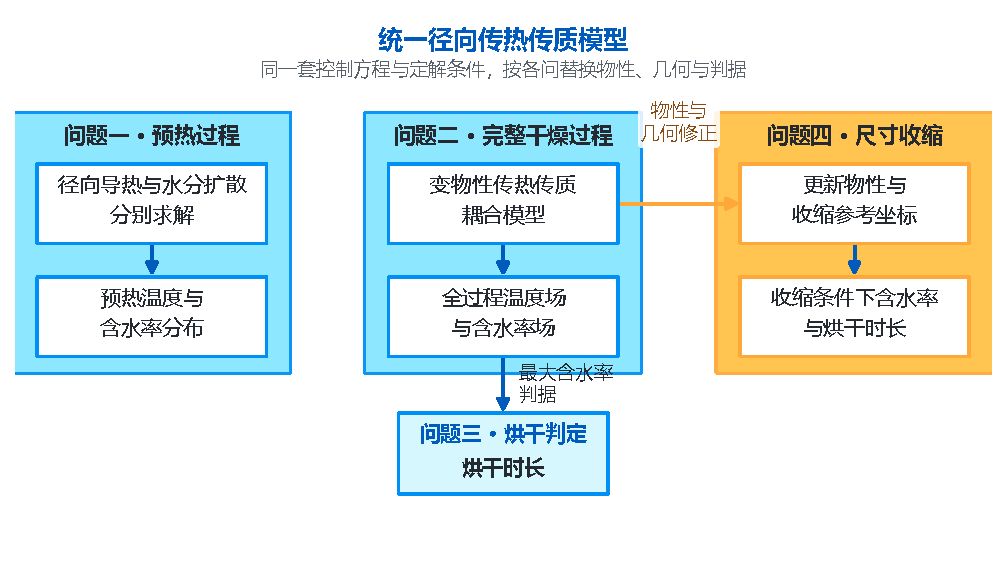
\includegraphics[width=\textwidth]{fig_relation.pdf}
\caption{四个问题与模型的关系：四问共用同一套径向传热传质模型；问题一为常物性预热特例，问题二为变物性完整过程；问题四在问题二模型上作物性与几何修正，问题三在问题二的结果上按最大含水率判据确定烘干时长。}
\label{fig:relation}
\end{figure}

\section{模型假设}

\begin{enumerate}[label=(H\arabic*),leftmargin=2.6em]
\item 圆柱、一维径向（中截面）模型，忽略端面与轴向梯度；问题一至三半径固定 $R_0$，问题四径向收缩、$L$ 固定。
\item 初始温度、含水率均匀（$T_0=\SI{28}{\celsius}$、$C_0=2.55$）；均匀各向同性连续介质。
\item 水分输运用题给有效扩散系数：$\partial_t C=\frac1r\partial_r(rD\partial_r C)$（问题四为物质导数形式），
不另列蒸汽/毛细/压力驱动项（不排除有效 $D$ 已含其净影响）。
\item Fourier 导热，$b(C)=\rho(C)c_p(C)$ 为\textbf{有效体积热容}：$\rho,c_p,k$ 保留题给经验物性的名称、公式与
数值作用；在给定几何与独立干物质基准的有效模型中，不额外把经验 $\rho(C)$ 与实测 $R(t)$ 同时作为精确
湿质量--体积闭合约束。不含水分携带显热、不含内部相变。
\item 传质第三类边界 $-D\partial_r C|_R=h_m(C_s-C_{\mathrm{env}})$，$C_{\mathrm{env}}(t)$ 取附件 1 数值为有效边界驱动；
初始角点（均匀初值零梯度而 $h_m(C_0-C_{\mathrm{env}}(0))\neq0$）作体内数据、Robin 自 $t>0$ 实施，不重置初值。
\item 传热第三类边界 $-k\partial_r T|_R=h(T_s-T_{\mathrm{air}})$；主线仅保留对流换热，不显式解析相变潜热。
\item 问题二至四沿用附录 2 的 $h,h_m$；问题一题给值不改。
\item 环境驱动：$0$--$\SI{14400}{s}$ 原始节点线性插值，$t>\SI{14400}{s}$ 取 $[10800,14400]\,\si{s}$ 内 61 点均值
（\SI{49.9989}{\celsius}、$0.049988$），$\SI{14400}{s}$ 登记为求解断点。
\item 中心零通量与正则性 $\partial_r C|_0=\partial_r T|_0=0$。
\item 问题四：$R(t)$ 由附件 2 线性插值，$t>\SI{72}{h}$ 保持 \SI{1.198}{cm} 并标注外推；仿射速度 $v_s=r\dot R/R$，
干物质均匀 $\rho_s(t)=\rho_{s0}(R_0/R)^2$。
\item 「烘干一般持续 2--3 天」仅为题面一般量级，既非终止条件也非拟合目标。
\end{enumerate}

\section{符号说明}

\begin{center}\small
\begin{tabular}{cll}
\toprule
符号 & 含义 & 单位 \\
\midrule
$r,\ t$ & 径向坐标、时间 & \si{m},\ \si{s} \\
$R_0,\ R(t)$ & 初始半径 \SI{0.02}{m}；问题四当前半径 & \si{m} \\
$L$ & 长度 \SI{0.25}{m}（固定） & \si{m} \\
$x=r/R(t)$ & 问题四参考坐标，$\in[0,1]$ & -- \\
$T,\ C$ & 温度、干基含水率 & \si{K}（输出 \si{\celsius}），\si{kg/kg} \\
$T_{\mathrm{air}}(t),\ C_{\mathrm{env}}(t)$ & 烘房温度、有效环境含水率 & \si{\celsius}$\to$\si{K},\ \si{kg/kg} \\
$\rho(C),c_p(C),k(C)$ & 题给经验物性 & \si{kg/m^3},\si{J/(kg.K)},\si{W/(m.K)} \\
$b(C)=\rho c_p$ & 有效体积热容 & \si{J/(m^3.K)} \\
$D(C)/D(C,T)$ & 题给有效扩散系数 & \si{m^2/s} \\
$h,\ h_m$ & 对流换热、传质系数 & \si{W/(m^2.K)},\ \si{m/s} \\
$\Cbar$ & 干基质量加权平均含水率 & \si{kg/kg} \\
$\Cmax(t)$ & 全域未舍入最大含水率（$=$ 节点最大值） & \si{kg/kg} \\
$\tstar,\ t_{\mathrm{sample}}$ & 阈值穿越时间；严格合格采样时刻 & \si{s}（报告 \si{h}） \\
$N,\ \Delta r,\ \Delta x$ & 网格区间数、步长 & -- \\
$Bi_h=hR/k,\ Bi_m=h_mR/D$ & 传热/传质 Biot 数 & -- \\
\bottomrule
\end{tabular}
\end{center}

\section{模型建立与求解}\label{sec:model}

四个问题共用一套沿半径方向的传热传质模型，只是物性、几何和判据不同。本节先建立共用的控制方程、定解条件与离散求解方法，再分问给出模型细节、求解结果与分析。

\subsection{共用控制方程与定解条件}\label{sec:gov}

在半径固定的问题一至三中，计算域为 $r\in[0,R_0]$。水分以有效扩散方式向外迁移，温度以导热方式传递，二者的守恒律写成散度形式
\begin{align}
\pd{C}{t} &= \frac{1}{r}\pd{}{r}\!\left(r\,D(C,T)\,\pd{C}{r}\right) \label{eq:govC}\\[2pt]
\rho(C)\,c_p(C)\,\pd{T}{t} &= \frac{1}{r}\pd{}{r}\!\left(r\,k(C)\,\pd{T}{r}\right) \label{eq:govT}
\end{align}
式~\eqref{eq:govC} 左端是含水率的变化率，右端是单位体积的净扩散流入；式~\eqref{eq:govT} 同理描述热量，其中 $\rho(C)c_p(C)$ 为有效体积热容。由于扩散系数 $D$ 与导热系数 $k$ 随状态在空间上变化，方程保留散度形式，使系数的空间变化被完整包含在通量里；若改写成 $D\,\nabla^2C$ 的形式，会遗漏系数梯度的贡献。式~\eqref{eq:govC} 中的 $T$ 取药材局部的热力学温度（$\si{K}$）。

初始时药材内部均匀，
\begin{equation}
T(r,0)=T_0=\SI{301.15}{K}\ (\SI{28}{\celsius}),\qquad C(r,0)=C_0=2.55
\label{eq:init}
\end{equation}
中心处由对称性有零梯度
\begin{equation}
\pd{C}{r}\bigg|_{r=0}=\pd{T}{r}\bigg|_{r=0}=0
\label{eq:center}
\end{equation}
表面 $r=R_0$ 处，向外的水分通量与热通量分别由传质、传热的第三类边界给出
\begin{equation}
-D(C_s,T_s)\,\pd{C}{r}\bigg|_{R_0}=h_m\big[C_s-\Cenv(t)\big],\qquad
-k(C_s)\,\pd{T}{r}\bigg|_{R_0}=h\big[T_s-\Tair(t)\big]
\label{eq:bc}
\end{equation}
其中 $C_s=C(R_0,t)$、$T_s=T(R_0,t)$ 为表面的含水率与温度。式~\eqref{eq:bc} 表示表面失水速率正比于表面与环境的含水浓度差，表面散热速率正比于表面与空气的温差。式~\eqref{eq:govC}--\eqref{eq:bc} 构成完整的定解问题。问题一是该问题组的特例：物性为常数、$D$ 只依赖含水率，于是式~\eqref{eq:govT} 不含 $C$、式~\eqref{eq:govC} 不含 $T$，温度与水分可以先后求解；问题二至四则需把二者作为耦合系统同时推进。

\subsection{节点型有限体积离散}\label{sec:fvm}

把半径区间 $[0,R_0]$ 均分为 $N$ 个小区间，得到 $N{+}1$ 个节点 $r_i=i\,\Delta r$（$i=0,1,\dots,N$，$\Delta r=R_0/N$）。中心和表面都取为节点：$r_0=0$ 为中心节点，$r_N=R_0$ 为表面节点，节点上的值即为要输出的温度和含水率。相邻节点之间的界面位于 $r_{i+1/2}=(i+\tfrac12)\Delta r$。围绕每个节点取一个控制体，对式~\eqref{eq:govC} 在控制体上积分，得到有限体积格式（图~\ref{fig:fvm}）。

\begin{figure}[H]\centering
\begin{tikzpicture}[font=\small,>=Stealth]
\def\dr{1.45}
\fill[palGold!30] ({1.5*\dr},-0.42) rectangle ({2.5*\dr},0.42);
\draw[palGold!60!black] ({1.5*\dr},-0.42) rectangle ({2.5*\dr},0.42);
\draw[thick,->] (-0.3,0) -- (8.9,0);
\node[anchor=west] at (8.95,0) {$r$};
\foreach \i in {0,1,2,3,4,5} {\fill[palBlueD] (\i*\dr,0) circle (2.4pt);}
\foreach \i in {0,1,2,3,4}{\draw[palRed,thick] ({(\i+0.5)*\dr},0.17)--({(\i+0.5)*\dr},-0.17);}
\node[anchor=south] at (0,0.10) {\scriptsize $r_0{=}0$};
\node[anchor=south] at (2*\dr,0.46) {\scriptsize 节点 $C_i,\,T_i$};
\node[anchor=south] at (5*\dr,0.10) {\scriptsize $r_N{=}R_0$};
\node[anchor=north,text=palBlueD] at (0,-0.22) {\scriptsize 中心节点};
\node[anchor=north,text=palBlueD] at (5*\dr,-0.22) {\scriptsize 表面节点};
\node[anchor=north,text=palGold!55!black] at (2*\dr,-0.46) {\scriptsize 控制体 $V_i$};
\node[anchor=north,text=palRed] at (2.5*\dr,-0.46) {\scriptsize 界面 $r_{i+1/2}$};
\draw[->,palRed,thick] (5*\dr,0.32) -- (5*\dr+0.95,0.32);
\node[anchor=south] at (5*\dr+0.55,0.44) {\scriptsize 表面交换 $h,\,h_m$};
\begin{scope}[yshift=-2.7cm]
\fill[palBlueL!35] (0,0.25) rectangle (3.2,0.45);
\draw[palBlueD] (0,0.25) rectangle (3.2,0.45);
\node[anchor=east] at (-0.1,0.35) {\scriptsize 物理域 $[0,R(t)]$};
\node[anchor=west] at (3.3,0.35) {\scriptsize $r=R(t)$};
\fill[palGold!25] (0,-0.45) rectangle (6.4,-0.25);
\draw[palGold!60!black] (0,-0.45) rectangle (6.4,-0.25);
\node[anchor=east] at (-0.1,-0.35) {\scriptsize 参考域 $[0,1]$};
\node[anchor=west] at (6.5,-0.35) {\scriptsize $x=1$};
\draw[->,palBlueD,thick] (3.2,0.22) -- (6.4,-0.22);
\node[anchor=west] at (4.9,0.02) {\scriptsize $x=r/R(t)$};
\end{scope}
\end{tikzpicture}
\caption{径向节点型有限体积离散（上）与问题四的参考坐标映射（下）。蓝点为节点、红色短线为界面、金色方块为一个控制体；下图中物理域 $[0,R(t)]$ 随时间收缩，映射到固定的参考域 $[0,1]$。}
\label{fig:fvm}
\end{figure}

对轴对称控制体积分后，各项都含有共同的几何因子 $2\pi L$；把它约去，界面上的面权重记为 $A_{i+1/2}=r_{i+1/2}$，控制体的体权重记为 $V_i=\int r\,\mathrm{d}r$（在各自控制体上积分）。内部节点 $V_i=r_i\Delta r$；中心控制体只占半个区间 $[0,\Delta r/2]$，为 $V_0=\Delta r^2/8$；表面控制体为 $V_N=R_0\Delta r/2-\Delta r^2/8$，三者满足
\begin{equation}
\sum_{i=0}^{N}V_i=\frac{R_0^2}{2}
\label{eq:vsum}
\end{equation}
这里的 $A_{i+1/2}$、$V_i$ 是约去 $2\pi L$ 后的权重，不是实际的面积和体积，只用于书写离散通量与守恒关系。界面上的水分通量（外向为正）取
\begin{equation}
F_{i+1/2}=-D_{i+1/2}\,\frac{C_{i+1}-C_i}{\Delta r}
\label{eq:flux}
\end{equation}
其中 $C_i$、$T_i$ 为节点值，$D_i=D(C_i,T_i)$、$k_i=k(C_i)$、$b_i=\rho(C_i)c_p(C_i)$ 为节点处的物性。界面扩散系数 $D_{i+1/2}$ 有两种取法：一是相邻两节点的\emph{调和平均} $D_{i+1/2}=2D_iD_{i+1}/(D_i+D_{i+1})$；二是沿界面对扩散系数作\emph{积分平均}
\begin{equation}
D^{\mathrm{I}}_{i+1/2}=\int_0^1 D\!\big((1-\xi)C_i+\xi C_{i+1},\ \bar T_{i+1/2}\big)\,\mathrm{d}\xi
\label{eq:integral}
\end{equation}
式中 $\xi\in[0,1]$ 是沿界面的积分变量，$\bar T_{i+1/2}=(T_i+T_{i+1})/2$ 是该界面两侧节点温度的局部平均（区别于整体平均温度），积分用 $8$ 点 Gauss 求积计算。已有研究指出，对强非线性扩散，简单的调和平均会在陡峭的干燥前沿附近引入数值偏差\cite{maddix2018a,maddix2018b}；积分平均在相邻两点扩散系数接近时能平滑退化、避免有效数字相消，长时间求解更稳定，故本文\textbf{正式计算采用积分界面}。

把通量代入并对控制体求和：内部节点 $1\le i\le N{-}1$ 满足
\begin{equation}
V_i\,\dot C_i=A_{i-1/2}F_{i-1/2}-A_{i+1/2}F_{i+1/2}
\label{eq:fvmint}
\end{equation}
中心节点没有左界面，只有右界面通量
\begin{equation}
V_0\,\dot C_0=-A_{1/2}F_{1/2}
\label{eq:fvmc}
\end{equation}
表面节点把式~\eqref{eq:bc} 的边界通量并入
\begin{equation}
V_N\,\dot C_N=A_{N-1/2}F_{N-1/2}-R_0\,h_m\big(C_N-\Cenv\big)
\label{eq:fvms}
\end{equation}
温度方程按相同方式离散，以 $b_iV_i$ 作时间导数的权重，导热系数在界面取调和平均，表面项为 $R_0\,h(T_N-\Tair)$。定义质量加权平均含水率 $\Cbar=\tfrac{2}{R_0^2}\sum_i V_iC_i$，由式~\eqref{eq:fvmint}--\eqref{eq:fvms} 求和可知它在半离散意义下精确满足
\begin{equation}
\frac{\mathrm{d}\Cbar}{\mathrm{d}t}=-\frac{2h_m}{R_0}\big(C_N-\Cenv\big)
\label{eq:massbal}
\end{equation}
即整体失水速率只由表面通量决定，这一关系将用于守恒检验。

\subsection{时间积分与求解流程}\label{sec:time}

离散后得到关于所有节点温度、含水率的常微分方程组，用两条互相印证的路线求解。

\textbf{向后 Euler（隐式，验证基线）：} 以固定时间步作向后 Euler 离散，装配矩阵时物性、半径等系数取当前步末的状态，每步用 Picard 迭代处理非线性直到相邻两次迭代之差小于容差。对线性化后的每一步，该格式无条件稳定；实际计算中还逐步核验了含水率不越出物理界限（第~\ref{sec:verification}~节）。其一阶时间精度便于做步长加密核验，故用作验证基线，但不据此断言非线性全过程的稳定性。

\textbf{BDF 自适应（正式计算）：} 长时间求解用变阶变步长的 BDF 方法（\texttt{scipy} 的 \texttt{solve\_ivp}）\cite{scipy}，相对容差取 $10^{-8}$。右端函数在每个求解时刻按当前时间 $t$ 取环境驱动与半径 $R(t)$；为提高效率，向求解器提供右端 Jacobian 的\textbf{稀疏结构}（块三对角），由其据此作有限差分近似。在环境数据的断点 $\SI{14400}{s}$ 处分段重启，使右端函数在断点两侧连续。求解流程可概括为：

\begin{enumerate}[label=\textbf{步骤 \arabic*.},leftmargin=3.4em,itemsep=1pt]
\item 读入几何、初值与对应附录的物性公式，按 $N$ 生成节点与控制体权重；
\item 由附件数据构造环境驱动 $\Tair(t)$、$\Cenv(t)$（问题四另构造半径 $R(t)$）；
\item 以初值 $(C_0,T_0)$ 为起点，用 BDF 向前积分式~\eqref{eq:fvmint}--\eqref{eq:fvms} 及温度方程，遇断点分段重启；
\item 对连续解在输出时刻重构全域场；对问题三、四追踪最大含水率并求其穿越 $0.15$ 的根；
\item 按题目要求的时间、位置网格采样，保留四位小数写出结果。
\end{enumerate}

数值上另作两点保护：当迭代中出现非物理的负含水率时把对应扩散系数置零并计数，指数项下溢时取零，均不直接裁剪状态量。

\subsection{环境驱动与半径输入}\label{sec:env}

环境驱动直接取自附件，不作改动。在 $0$ 至 $\SI{14400}{s}$（$\SI{4}{h}$）内，空气温度和环境含水浓度按附件 1 的原始节点分段线性插值；超过 $\SI{4}{h}$ 后附件不再提供数据，取最后一小时窗口 $[10800,14400]\,\si{s}$ 内 $61$ 个样本的算术平均作为常值延续，得 $\Tair\approx\SI{49.999}{\celsius}$、$\Cenv\approx0.04999$，并把 $\SI{14400}{s}$ 记为求解断点。问题四的半径按附件 2 分段线性插值，$\SI{72}{h}$ 之后保持末值 $\SI{1.198}{cm}$。三条输入曲线及其外推段见图~\ref{fig:inputs}。

\begin{figure}[H]\centering
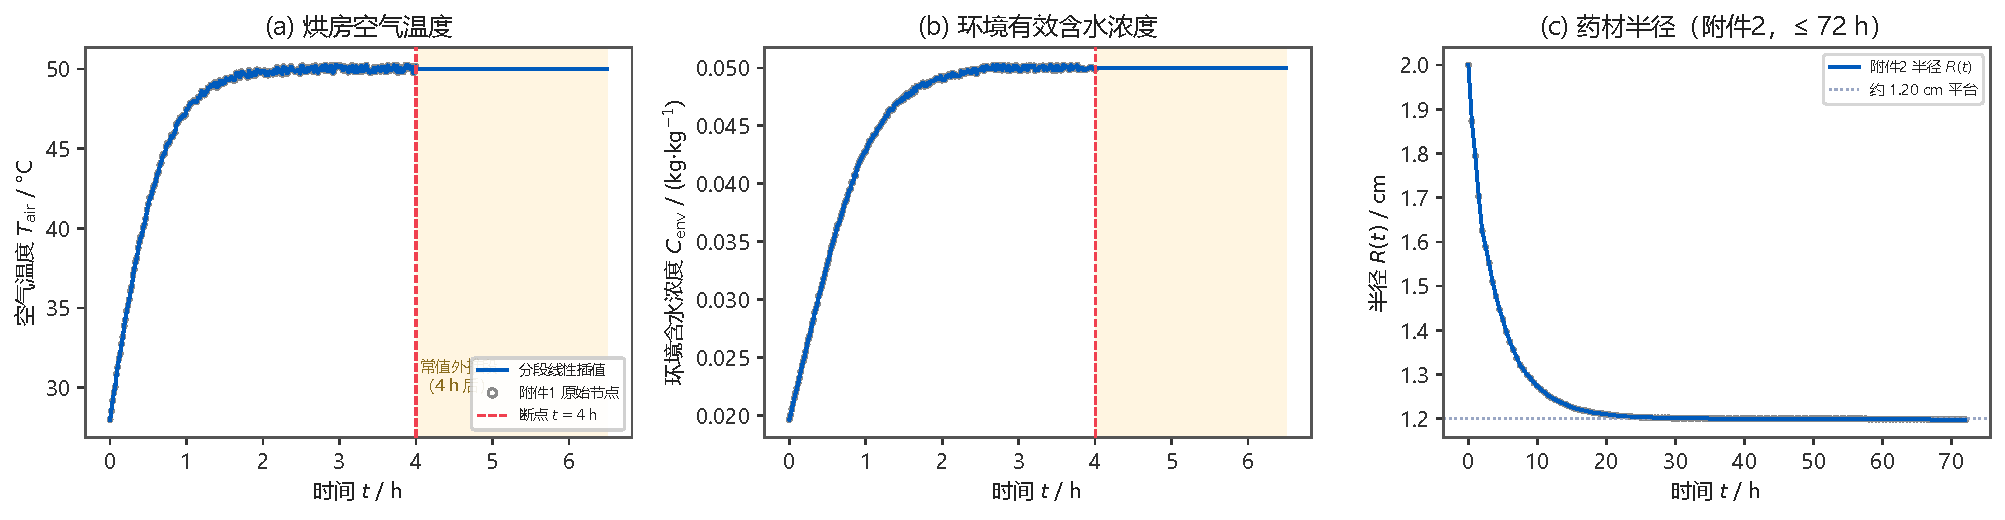
\includegraphics[width=\textwidth]{fig_inputs.pdf}
\caption{环境与半径输入：灰圈为附件原始节点，蓝线为分段线性插值，金色区域为常值外推段，(a)(b) 中红色虚线为 $\SI{4}{h}$ 断点。}
\label{fig:inputs}
\end{figure}

\subsection{问题一：预热阶段（附录 2）}\label{sec:q1}

\textbf{建模思路：} 问题一给出常物性与只依赖含水率的扩散系数，
\begin{equation}
\rho=\SI{820}{kg/m^3},\quad c_p=\SI{2600}{J/(kg.K)},\quad k=\SI{0.36}{W/(m.K)},\quad
D(C)=7\times10^{-9}\,e^{-0.89/C}\ \si{m^2/s}
\label{eq:props1}
\end{equation}
式中 $C$ 无量纲。此时温度方程与水分方程解耦，可先解温度、再解水分。预热阶段仅 $\SI{1800}{s}$，表面附近水分开始向外迁移，梯度很陡，是求解的重点。

\textbf{模型建立：} 沿用式~\eqref{eq:govC}--\eqref{eq:bc}，其中物性取式~\eqref{eq:props1}。表面传热、传质 Biot 数分别约为 $Bi_h=1.39$、$Bi_m=3.24$，说明表面交换与内部输运快慢相当，边界层不可忽略。

\textbf{求解方法：} 按第~\ref{sec:time}~节的 BDF 流程求解。由于早期表面层厚度约 $\sqrt{Dt}$ 小于粗网格步长，需较密的网格才能分辨表面梯度，正式计算取 $N=1600$（依据见第~\ref{sec:verification}~节的网格收敛）。在 $0$ 至 $\SI{1800}{s}$ 内每 $\SI{1}{s}$、每 $\SI{0.1}{cm}$ 输出温度与含水率。

\textbf{求解结果：} 不同时刻的径向剖面见图~\ref{fig:q1}，代表性数值见表~\ref{tab:t1}、表~\ref{tab:t2}。

\begin{figure}[H]\centering
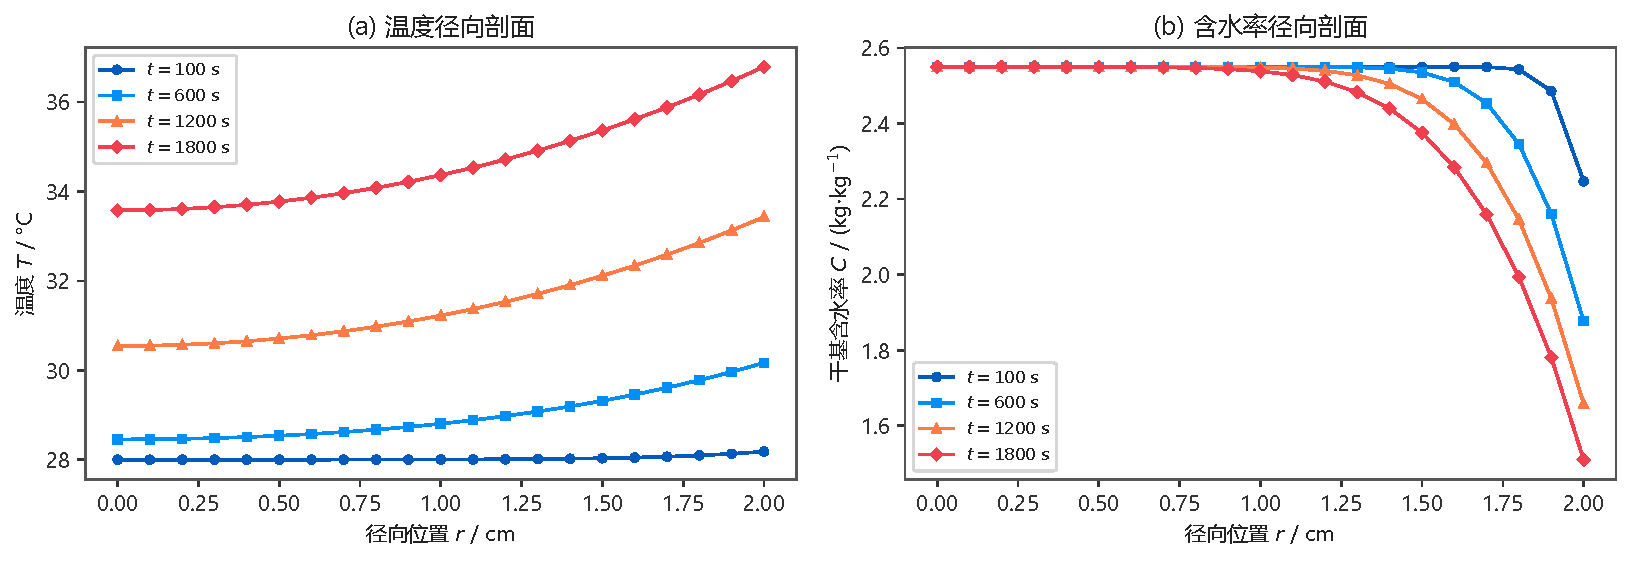
\includegraphics[width=0.94\textwidth]{fig_q1_profiles.pdf}
\caption{问题一不同时刻的径向温度剖面（左）与含水率剖面（右）；同一时刻在两幅子图中用同一颜色与标记。}
\label{fig:q1}
\end{figure}

\begin{table}[H]\centering\small
\caption{问题一温度场 $T$（$\si{\celsius}$，横向为到药材中心的距离 $r/\si{cm}$）}\label{tab:t1}
\input{tables/table1}
\end{table}
\begin{table}[H]\centering\small
\caption{问题一含水率场 $C$（$\si{kg/kg}$，干基；横向为 $r/\si{cm}$）}\label{tab:t2}
\input{tables/table2}
\end{table}

\textbf{结果分析与检验：} 在 $\SI{1800}{s}$ 时，中心温度为 $\SI{33.5754}{\celsius}$、表面温度为 $\SI{36.7856}{\celsius}$，相差约 $\SI{3.21}{\celsius}$。中心已从 $\SI{28}{\celsius}$ 升到 $\SI{33.58}{\celsius}$，说明预热末期径向温度尚未达到均衡，仍在继续升温。同一时刻表面干基含水率已从 $2.55$ 降到 $1.5102$，而中心含水率仍为 $2.5500$、几乎等于初值。可见预热阶段的失水几乎全部发生在靠近表面的薄层，中心还没有开始明显干燥；图~\ref{fig:q1} 右图中含水率剖面自表面向内迅速抬升、在约 $r=\SI{1}{cm}$ 以内几乎水平，正体现了这一边界层特征。本问展示的是附录 2 条件下的预热规律；问题二至四从题给初始状态（式~\eqref{eq:init}）起统一使用各自附录的物性，并不把问题一的末状态接作后续问题的初值。

\subsection{问题二与问题三：完整过程与达标判定（附录 3）}\label{sec:q23}

\textbf{建模思路：} 问题二需要描述温度与含水率在整个干燥过程中的共同演化。含水率改变材料的导热系数与体积热容，温度又通过扩散系数影响水分迁移，因此把两类控制方程组成耦合系统同时求解。对该系统完成数值求解后，问题三不再引入新的状态方程，而是以全径向域最大含水率构造终止判据，从同一数值解确定干燥时长。

\textbf{模型建立：} 控制方程与边界仍为式~\eqref{eq:govC}--\eqref{eq:bc}，但物性取附录 3 随状态变化的形式
\begin{align}
\rho(C)&=650+128\,C,\qquad c_p(C)=1450+2736\,\frac{C}{C+1}\label{eq:props3a}\\
k(C)&=0.21+0.38\,\frac{C}{C+1},\qquad D(C,T)=2.4\times10^{-3}\,e^{-0.45/C}\,e^{-3850/T}\ \si{m^2/s}\label{eq:props3b}
\end{align}
其中密度、比热、导热系数的单位分别为 $\si{kg/m^3}$、$\si{J/(kg.K)}$、$\si{W/(m.K)}$，含水率 $C$ 无量纲，扩散系数中的温度 $T$ 以 $\si{K}$ 计。达标判据「各处含水率低于 $0.15$」等价于最大含水率低于 $0.15$；该最大值定义为所有节点（或重构径向场）上的最大值，本算例中它位于中心节点。

\textbf{求解方法：} 按第~\ref{sec:time}~节的耦合 BDF 流程从初值一次积分到干燥后期，正式计算取 $N=800$。问题二每 $\SI{1}{s}$ 输出全场。问题三在同一条连续解上求最大含水率满足 $\Cmax(t)=0.15$ 的根，得到\textbf{阈值穿越时间} $\tstar$。为区分两个相近的时间量：$\tstar$ 是由连续解求根得到的严格达标时刻的下确界；而在按每 $\SI{60}{s}$ 输出的结果里，首个计算得到的、最大含水率低于 $0.15$ 的输出时刻记为 $\tsamp$，用于结果文件的末行。由于失水单调、且常数 $0.15$ 在无源方程上是一个上解，最大含水率一旦降到 $0.15$ 以下便不再回升，故 $\tsamp\ge\tstar$ 且二者相差不足 $\SI{60}{s}$。

\textbf{求解结果：} 温度场与含水率场的演化见图~\ref{fig:q23}，问题二的代表性数值见表~\ref{tab:t3}、表~\ref{tab:t4}，问题三达标前的含水率见表~\ref{tab:t5}。求得达标时长
\begin{equation}
\tstar_3=\SI{57.4740}{h}\ (\SI{206906.5}{s}),\qquad \tsampq{3}=\SI{206940}{s}
\label{eq:tstar3}
\end{equation}

\begin{figure}[H]\centering
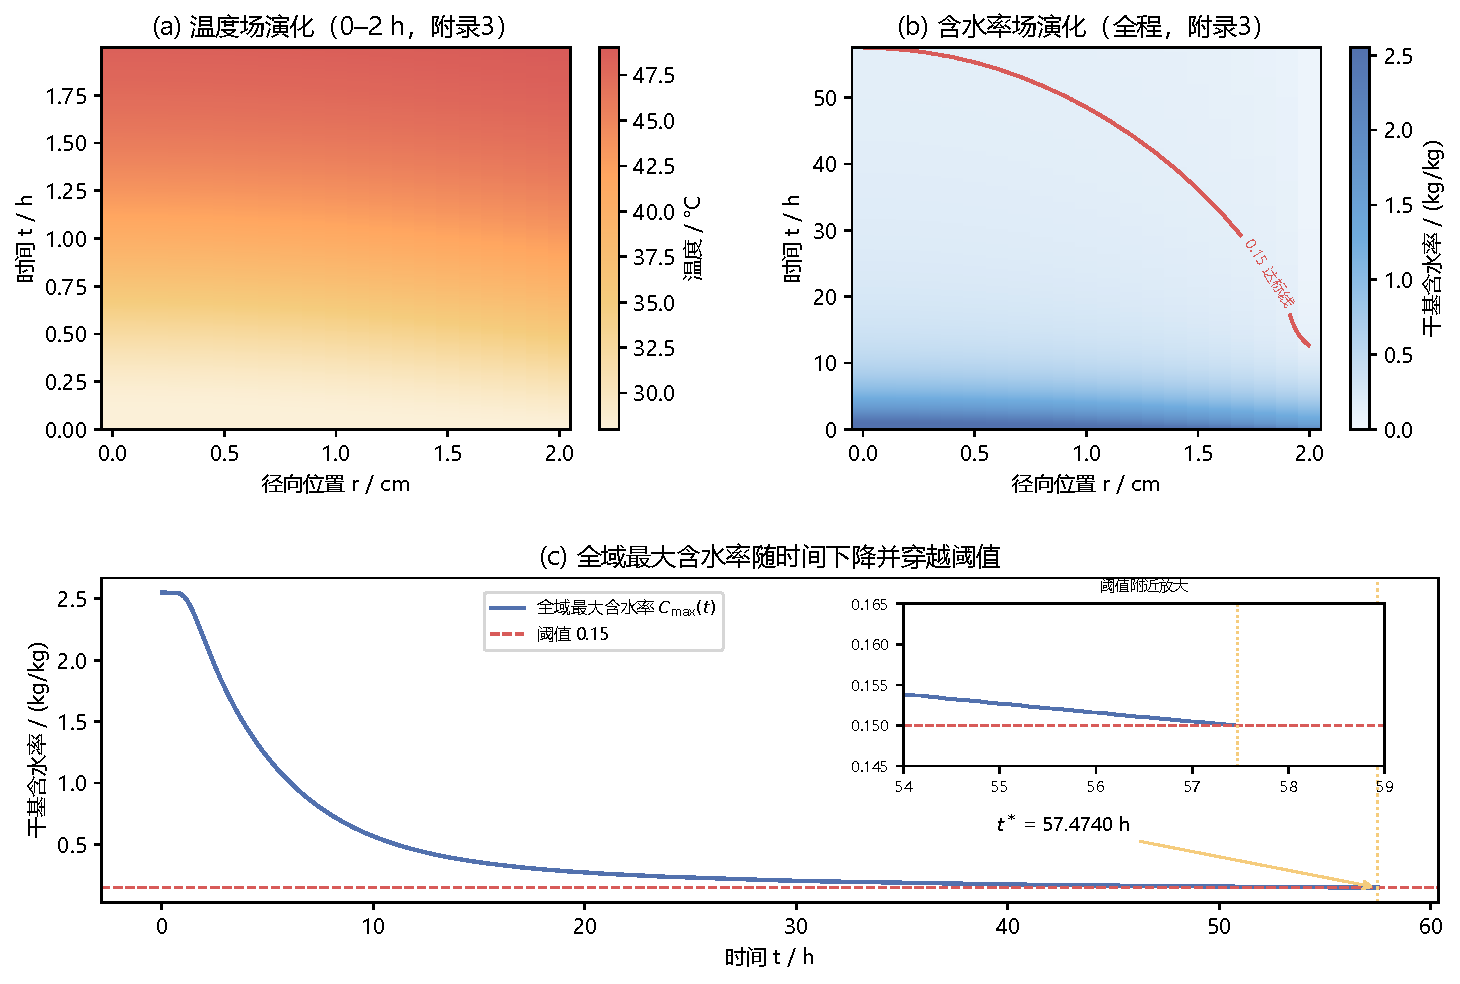
\includegraphics[width=0.98\textwidth]{fig_q23_fields.pdf}
\caption{问题二、三：温度场在前 $\SI{2}{h}$ 的演化（a）、含水率场全程演化及 $0.15$ 达标线（b）、以及输出最大含水率随时间的下降（c）；温度与含水率使用各自独立的色标与单位，(c) 的放大窗只示 $\SI{60}{s}$、四位小数的采样分辨率，严格达标时刻由未舍入求根确定。}
\label{fig:q23}
\end{figure}

\begin{table}[H]\centering\small
\caption{问题二温度场 $T$（$\si{\celsius}$，$0.5$--$\SI{3}{h}$；横向为 $r/\si{cm}$）}\label{tab:t3}
\input{tables/table3}
\end{table}
\begin{table}[H]\centering\small
\caption{问题二含水率场 $C$（$\si{kg/kg}$，$0.5$--$\SI{3}{h}$；横向为 $r/\si{cm}$）}\label{tab:t4}
\input{tables/table4}
\end{table}
\begin{table}[H]\centering\small
\caption{问题三达标前含水率 $C$（每 $\SI{6}{h}$，末行为达标时刻 $\tstar_3=\SI{57.4740}{h}$；横向为 $r/\si{cm}$）}\label{tab:t5}
\input{tables/table5}
\end{table}

\textbf{结果分析与检验：} 温度与水分呈现出不同的时间尺度。烘干 $\SI{3}{h}$ 时，中心与表面的温度分别为 $\SI{49.8495}{\celsius}$、$\SI{49.9664}{\celsius}$，相差仅约 $\SI{0.1169}{\celsius}$，温度分布已接近均匀并逼近热风温度；而同一时刻中心与表面的干基含水率分别为 $1.7662$ 和 $1.0081$，仍存在明显梯度。这表明热量在数小时内即传遍断面，水分的均匀化却慢得多，干燥的快慢主要由水分迁移决定。图~\ref{fig:q23}(b) 中含水率由外向内逐层降低，$0.15$ 达标线最后才到达中心；图~\ref{fig:q23}(c) 显示输出最大含水率单调下降，其穿越 $0.15$ 的时刻由未舍入求根确定为 $\tstar_3$。表~\ref{tab:t5} 末行对应 $\tstar_3$，此刻中心未舍入含水率恰为 $0.15$、四位小数显示为 $0.1500$，严格低于 $0.15$ 出现在这一时刻之后的瞬间；达标判定以未舍入的最大含水率为准，不以四位小数平台作依据。结合网格与时间加密的收敛核验（第~\ref{sec:verification}~节），该达标时长在所设数值容差内可靠。

\subsection{问题四：尺寸收缩情形（附录 4）}\label{sec:q4}

\textbf{建模思路：} 药材在干燥中失水收缩，半径从 $\SI{2.0}{cm}$ 缩小到约 $\SI{1.2}{cm}$。计算域本身随时间变化，若在物理坐标上直接求解，动边界会带来附加对流项且需反复重划网格。为此引入随物料一起收缩的参考坐标 $x=r/R(t)$，把方程变换到固定的单位区间 $x\in[0,1]$ 上求解。

\textbf{模型建立：} 设参考坐标下的温度、含水率为 $\tilde T(x,t)$、$\tilde c(x,t)$，满足 $\tilde c(x,t)=C(xR(t),t)$。物料各点随边界仿射收缩，$r=xR(t)$，故物质点速度与径向导数为
\begin{equation}
v_s=\pd{r}{t}\bigg|_{x}=x\dot R=\frac{\dot R}{R}\,r,\qquad \pd{}{r}=\frac1R\pd{}{x}
\label{eq:q4kin}
\end{equation}
同一含水率场在固定物理坐标与固定参考坐标下的时间导数相差一个随动对流项
\begin{equation}
\pd{\tilde c}{t}\bigg|_{x}=\pd{C}{t}\bigg|_{r}+v_s\,\pd{C}{r}
\label{eq:q4mat}
\end{equation}
把物理方程 $\left.\partial_t C\right|_r=\tfrac1r\partial_r(rD\partial_r C)$ 代入式~\eqref{eq:q4mat}，并利用式~\eqref{eq:q4kin} 的仿射速度使随动对流与坐标缩放恰好相抵，方程中不再显含收缩速度 $\dot R$，只剩下半径 $R(t)$
\begin{equation}
\pd{\tilde c}{t}=\frac{1}{R^2 x}\pd{}{x}\!\left(x\,D(\tilde c,\tilde T)\,\pd{\tilde c}{x}\right),\qquad
b(\tilde c)\pd{\tilde T}{t}=\frac{1}{R^2 x}\pd{}{x}\!\left(x\,k(\tilde c)\,\pd{\tilde T}{x}\right)
\label{eq:q4gov}
\end{equation}
可见内部扩散被 $1/R^2$ 加快、表面交换被 $1/R$ 放大。仿射假设是这一化简的关键：只有当网格速度等于物料速度 $v_s=(\dot R/R)r$ 时相对对流才恰好相消，任意换一个坐标都不会自动消去。参考域上的初始与中心条件由式~\eqref{eq:init}、\eqref{eq:center} 平移而来（$\tilde T(x,0)=T_0$、$\tilde c(x,0)=C_0$，中心 $x=0$ 处零梯度），表面 $x=1$ 处的边界为
\begin{equation}
-\frac{D}{R}\pd{\tilde c}{x}\bigg|_{x=1}=h_m\big[\tilde c(1,t)-\Cenv\big],\qquad
-\frac{k}{R}\pd{\tilde T}{x}\bigg|_{x=1}=h\big[\tilde T(1,t)-\Tair\big]
\label{eq:q4bc}
\end{equation}
物性取附录 4 的形式
\begin{align}
\rho(\tilde c)&=760+90\,\tilde c,\qquad c_p(\tilde c)=1850+2150\,\frac{\tilde c}{\tilde c+1}\label{eq:props4a}\\
k(\tilde c)&=0.12+0.20\,\frac{\tilde c}{\tilde c+1},\qquad D(\tilde c,\tilde T)=4.2\times10^{-4}\,e^{-0.30/\tilde c}\,e^{-3850/\tilde T}\ \si{m^2/s}\label{eq:props4b}
\end{align}
单位约定同式~\eqref{eq:props3a}--\eqref{eq:props3b}，扩散系数中的温度 $\tilde T$ 以 $\si{K}$ 计。由干物质守恒，干物质基准密度随收缩按 $\rhos(t)=\rho_{\mathrm{s}0}(R_0/R(t))^2$ 变化。

\textbf{求解方法：} 在参考坐标上按第~\ref{sec:time}~节的耦合 BDF 流程求解式~\eqref{eq:q4gov}--\eqref{eq:q4bc}，正式计算取 $N=800$，右端在每个求解时刻按当前 $R(t)$ 取值。离散后表面节点记为 $N$，其值即 $\tilde c(1,t)$。输出时把固定物理位置 $r_j=0.1j\,\si{cm}$ 映射回参考坐标 $x_j(t)=r_j/R(t)$：当 $x_j\le1$ 时由节点线性插值得到该处含水率，当 $r_j$ 落在收缩后的表面之外时该位置已不属于药材，输出留空。

\textbf{求解结果：} 含水率场与移动边界、以及固定位置和表面的时程见图~\ref{fig:q4}，代表性数值见表~\ref{tab:t6}，各行对应的半径见表~\ref{tab:t6r}。求得达标时长
\begin{equation}
\tstar_4=\SI{51.0920}{h}\ (\SI{183931.3}{s}),\qquad R(\tstar_4)=\SI{1.20}{cm}
\label{eq:tstar4}
\end{equation}
达标时刻对应的半径仍在附件 2 的 $\SI{72}{h}$ 数据范围内，故\textbf{结果不依赖半径的外推段}（但仍依赖 $\SI{4}{h}$ 之后的环境常值外推）。

\begin{figure}[H]\centering
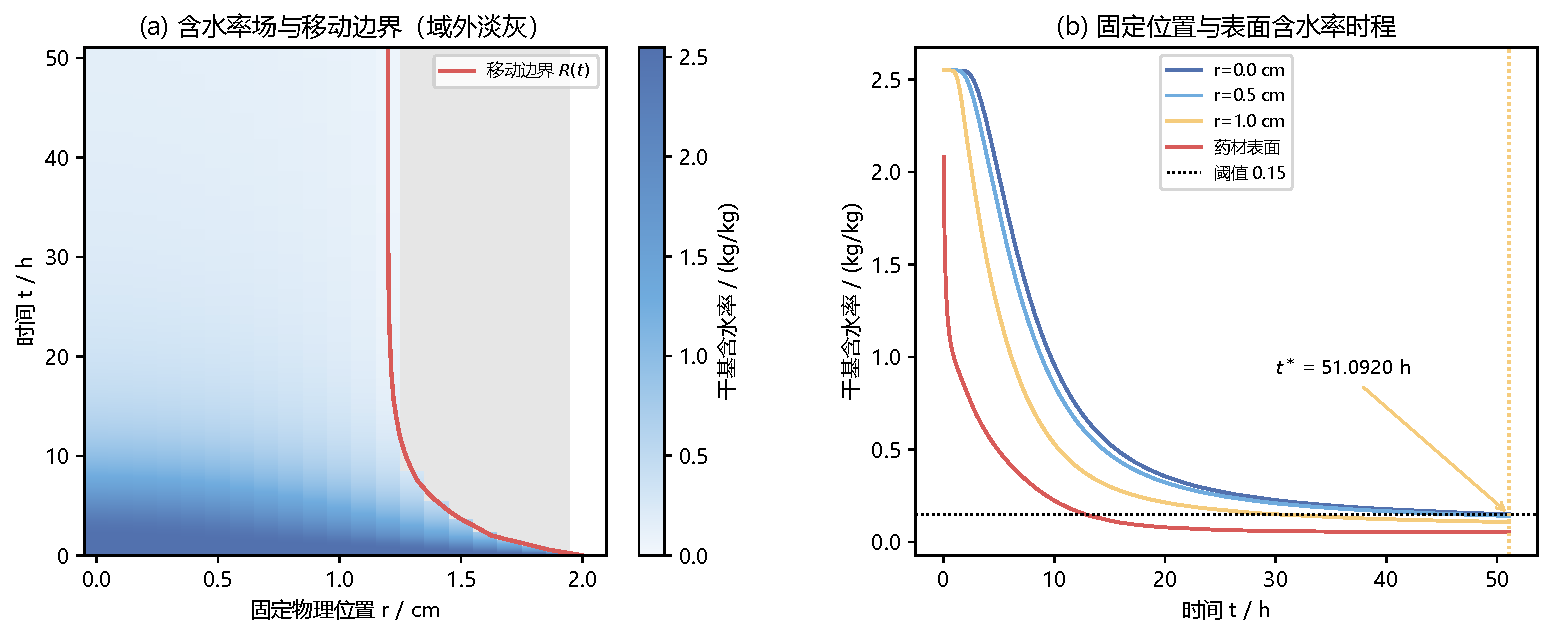
\includegraphics[width=\textwidth]{fig_q4_fields.pdf}
\caption{问题四：含水率场与移动边界 $R(t)$（a，域外以淡灰表示、场严格裁切到 $r\le R(t)$），以及固定位置与表面的含水率时程（b，含首末输出行，事件时刻 $\tstar_4$ 标注）。}
\label{fig:q4}
\end{figure}

\begin{table}[H]\centering\small
\begin{minipage}[t]{0.60\textwidth}\centering
\caption{问题四含水率（$\si{kg/kg}$，末行为 $\tstar_4=\SI{51.0920}{h}$；横向为固定位置 $r/\si{cm}$）}\label{tab:t6}
\begin{tabular}{ccccc}
\toprule
$t$/h & $r{=}0$ & $r{=}0.5$ & $r{=}1.0$ & 药材表面 \\
\midrule
6.0000 & 1.7196 & 1.5378 & 1.0226 & 0.4207 \\
12.0000 & 0.7377 & 0.6546 & 0.4083 & 0.1669 \\
18.0000 & 0.4088 & 0.3687 & 0.2397 & 0.0892 \\
24.0000 & 0.2851 & 0.2611 & 0.1790 & 0.0673 \\
30.0000 & 0.2263 & 0.2094 & 0.1493 & 0.0595 \\
36.0000 & 0.1928 & 0.1797 & 0.1317 & 0.0560 \\
42.0000 & 0.1712 & 0.1604 & 0.1200 & 0.0541 \\
48.0000 & 0.1561 & 0.1468 & 0.1116 & 0.0530 \\
51.0920 & 0.1500 & 0.1413 & 0.1081 & 0.0526 \\
\bottomrule
\end{tabular}
\end{minipage}\hfill
\begin{minipage}[t]{0.36\textwidth}\centering
\caption{问题四各行对应半径 $R(t)$}\label{tab:t6r}
\begin{tabular}{ccc}
\toprule
$t$/h & $R$/cm & 外推 \\
\midrule
6.0000 & 1.3740 & 否 \\
12.0000 & 1.2480 & 否 \\
18.0000 & 1.2140 & 否 \\
24.0000 & 1.2040 & 否 \\
30.0000 & 1.2010 & 否 \\
36.0000 & 1.2000 & 否 \\
42.0000 & 1.2000 & 否 \\
48.0000 & 1.2000 & 否 \\
51.0920 & 1.2000 & 否 \\
\bottomrule
\end{tabular}
\end{minipage}
\end{table}

表~\ref{tab:t6} 中固定位置 $r=1.5$、$\SI{2.0}{cm}$ 在 $t\ge\SI{6}{h}$ 时已位于收缩后的表面之外（域外），故不列出；域外为空表示该处不再属于药材，并非含水率为零。

\textbf{结果分析与检验：} 图~\ref{fig:q4}(a) 中移动边界 $R(t)$ 先快后慢地内移并在约 $\SI{1.2}{cm}$ 处趋于平稳，边界以外的位置逐渐脱离药材；固定厘米位置的时程（图~\ref{fig:q4}(b)）与表面时程不同，越靠外的位置越早被边界越过。要理解收缩对干燥时间的作用，需把物性变化和几何收缩分开。为此另算「附录 4 物性、半径固定为 $R_0$」的对照情形，与「附录 3 物性、半径固定」「附录 4 物性、半径收缩」在同一网格（$N=400$）上比较，三者达标时长分别约为 $\SI{57.47}{h}$、$\SI{129.85}{h}$、$\SI{51.09}{h}$（详见第~\ref{sec:verification}~节图~\ref{fig:threecase}）。由此可见，把物性从附录 3 换成附录 4 会显著\emph{延长}干燥，而尺寸收缩又把干燥\emph{缩短}。因此，问题三到问题四达标时间的变化是这两种相反效应叠加的结果，不能简单地全部归因于收缩。需说明的是，这里的三情形对照是沿所选建模路径的条件比较，并非完整的双因素交互分解。

\section{模型检验与灵敏度分析}\label{sec:ver}
\label{sec:verification}

全部检验由统一代码实测生成，判据与验证一律用未舍入值。

\paragraph{解析解对照（V-1/V-2）.}
以常物性、恒环境构造圆柱第三类边界瞬态级数解 $\theta=\sum_n c_nJ_0(\lambda_n\eta)e^{-\lambda_n^2Fo}$
（特征方程 $\lambda_nJ_1(\lambda_n)=Bi\,J_0(\lambda_n)$）。\textbf{分离空间阶与时间阶}：半离散（紧容差 BDF）
vs 级数解，$N=200/400/800$ 表面点热误差 $7.57/1.89/0.47\times10^{-5}\,\si{\celsius}$（\textbf{二阶}）；
固定细网格 BE $\Delta t=1/0.5/0.25\,\si{s}$ 一阶。

\paragraph{网格与界面收敛（V-3/V-11）.}
界面系数对照见图 \ref{fig:conv}：调和平均 $N=200/400/800$ 得
$\tstar=58.96/57.69/57.51\,\si{h}$（$N{=}200{\to}400$ 差 \SI{1.27}{h}），
积分界面 $57.4745/57.4741/57.4740\,\si{h}$（收敛显著更优），故生产采用积分界面。
按\textbf{各问实际场点误差}（生产 $N$ vs 更细 $N$，同 rtol）选定最终网格：问题一 $N{=}1600$（vs $3200$，
全 1800 行最大 $|\Delta C|=\num{4.69e-5}$、$|\Delta T|=\SI{2.23e-4}{\celsius}$）；问题二/三 $N{=}800$
（vs $1600$，全 \num{206907} 逐秒行 $|\Delta C|=\num{1.55e-4}$）；问题四 $N{=}800$（vs $1600$，全 \num{3066}
分钟行 $|\Delta|=\num{2.19e-4}$，最差恰在 $r=\SI{1.2}{cm}$，独立登记，不以 $\tstar$ 收敛替代场点验收）。
均低于门槛 $\Delta C{<}\num{5e-4}$、$\Delta T{<}\SI{1e-2}{\celsius}$。独立时间加密（rtol $10^{-8}$ vs $10^{-10}$）
$\Delta\tstar<\num{1e-7}\,\si{h}$；8 vs 16 点界面求积 $\Delta\tstar<\num{7e-7}\,\si{h}$。

\begin{figure}[H]\centering
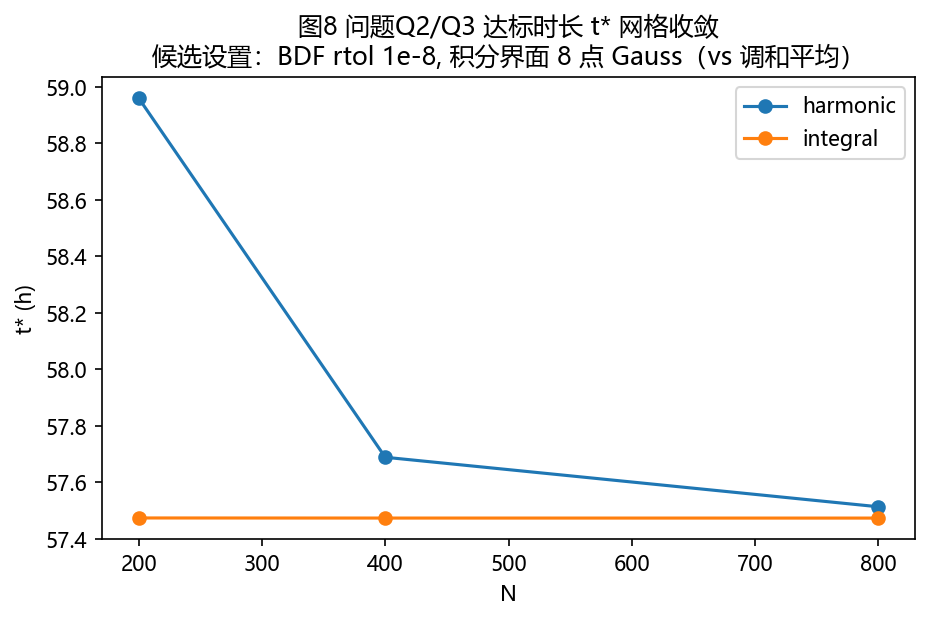
\includegraphics[width=0.72\textwidth]{fig8_convergence.png}
\caption{问题二/三达标时长 $\tstar$ 网格收敛：积分界面（平坦）vs 调和平均。}
\label{fig:conv}
\end{figure}

\paragraph{守恒与物理界限（V-4/V-5/V-10）.}
BE 离散代数收支 $|\Cbar_N-\Cbar_0+I_{BE}|/|\Delta\Cbar|\approx\num{1.5e-14}$（\emph{恒等式，非时间精度}）；
独立连续通量梯形求积与理论差 $\tfrac{\Delta t}{2}(f_0-f_N)$ 逐位一致，粗步 $\Delta t{=}\SI{1}{s}$ 相对差
$\num{1.64e-4}$（$>10^{-4}$ 门槛，粗步未过）、细步 $\Delta t{=}\SI{0.25}{s}$ $\num{4.11e-5}$（细步通过）；
BDF 独立自适应求积相对差 $\num{9.3e-9}\le10\,\mathrm{rtol}$。有效热残差（\si{W/m} 口径）$\num{3.2e-10}$。
物理界限包络（接受解落在历史 $[C_{lo},C_{hi}]$、$[T_{lo},T_{hi}]$）无越界。静态极限（$R\equiv R_0$ 动域 vs
固定域求解器）相对差 $\num{3.6e-8}$。

\paragraph{附录 4 固定半径对照（S10）.}
为分离物性与几何效应，增设「附录 4 $+$ 固定 $R_0$」对照，与「附录 3/$R_0$」「附录 4/$R(t)$」构成三情形
（图 \ref{fig:s10}）：$\tstar$ 分别约 $57.47/129.85/51.09\,\si{h}$。物性变化（$\text{①}\to\text{②}$，时长升）
与尺寸收缩（$\text{②}\to\text{③}$，时长降）方向相反，故\textbf{不可把问题三到四的差异全部归为收缩}。

\begin{figure}[H]\centering

\includegraphics[width=0.7\textwidth]{fig10_s10.png}
\caption{附录 4 固定半径对照：分离物性与几何效应（三情形 $\tstar$ vs $N$）。}
\label{fig:s10}
\end{figure}

\paragraph{灵敏度分析（S1--S6）.}
以问题二/三为基线，每情景重新积分。传质系数 $h_m\times0.5/2$ 使 $\tstar$ 变化 $+7.46/-2.80\,\si{h}$（影响最大）；
换热系数 $h$ 影响小（$\pm0.04$--$0.08\,\si{h}$）；外推温度 $\pm\SI{0.39}{\celsius}$ 使 $\tstar$ 变 $\mp0.71\,\si{h}$；
数据平滑 \texttt{smooth121} 变化 $<\SI{0.02}{h}$（未分辨）。数值误差小于所报情景差，结论可分辨。

\section{模型评价与推广}\label{sec:eval}

\paragraph{优点.}
(i) 四问共用同一套散度形式非线性方程与节点型有限体积离散，物理主线一致、可追溯；
(ii) 达标判据在未舍入全域重构场上连续求根，区分阈值穿越时间 $\tstar$ 与严格合格采样时刻，
避免四位小数显示的伪精度；(iii) 问题四以参考坐标处理动边界，方程只含 $R(t)$，守恒离散精确；
(iv) 数值配置由各问实际场点误差选定并登记，界面系数、时间格式、网格均通过独立检验。

\paragraph{局限：端面效应（V-15 增量校核）.}
一维径向近似忽略端面。以线性常系数、恒环境阶跃辅助问题（乘积解 $\theta_{\mathrm{finite}}=\theta_{\mathrm{radial}}
\theta_{\mathrm{slab}}$，平板半厚 $L/2=\SI{0.125}{m}$）估计端面\textbf{增量} $\Delta T=(T_0-T_\infty)
\theta_{\mathrm{radial}}(\theta_{\mathrm{slab}}-1)$（质同理），在问题一至四\emph{全部相关表点时刻/位置}
（含问题二表 3/4 的 $0.5$--$\SI{3}{h}$）评估：最大 $|\Delta T|=\SI{9.1013e-4}{\celsius}$（位于 $\SI{1.5}{h}$、$r=0$）、
$|\Delta C|=\num{1.1281e-5}$（位于 $\SI{42}{h}$、$r=0$），均远低于 $\SI{0.1}{\celsius}$、$0.005$。
$|\Delta C|$ 随平板本征项数 $\text{nterms}=60/120/200$ 收敛于 $\num{1.13e-5}$（$60$ 项时的 $\num{4.76e-4}$
系小 $Fo$ 级数截断底噪，非物理值），故报告值为物理增量。\textbf{该结论仅限固定物性、固定环境的线性辅助
模型及已检查位置/时刻，不认证/否定变物性时变环境的非线性主线。} 机理：轴向扩散时间尺度
$(L/2)^2/D\approx\SI{886}{h}$ 远大于径向 $R_0^2/D\approx\SI{22.7}{h}$，端面显现时径向场已趋均衡，
故乘积增量极小。

\paragraph{其他局限.}
本文采用题给有效传热传质模型，未显式解析相变潜热；更完整机理模型需要一致的界面平衡及材料参数，
超出本题给定信息。烘房「水分浓度」作为有效边界驱动 $C_{\mathrm{env}}$，非已识别的真实平衡含水率；
$h,h_m$ 跨问沿用为额外有效系数假设。$\SI{4}{h}$ 后环境与 $\SI{72}{h}$ 后半径均为外推，已显式标注。

\paragraph{推广.}
模型框架可推广到其他细长物料的对流干燥：更换经验物性组、边界系数与几何驱动即可；
积分界面系数对陡峭扩散前沿的稳健性、参考坐标对给定收缩轨迹的处理，适用于一类含强非线性扩散与
动边界的干燥/浸出问题。若获得材料吸附--解吸等温线与相变参数，可在现框架上增补平衡边界与潜热汇。


\section*{AI 工具使用声明}

本参赛队在完成本文过程中使用了 AI 工具，主要用于文献与资料的检索梳理、数值方法与程序实现的辅助、以及文字表达的润色。模型的建立、方程与边界条件的选取、达标判据的设计、数值方案的确定以及全部结论，均由参赛队主导完成；AI 生成的内容经参赛队逐项复算与核对后才予采用，未经核对者不作为结论。文中所有正式数值结果（温度场、含水率场、达标时长以及表~1--6）由参赛队统一的程序在既定环境下运行得到，复现所需的命令、配置与源程序见附录。AI 工具使用的具体情况按竞赛规定\cite{mcmrule}随支撑材料一并提交。


% 参考文献按正文首次引用顺序排列（thebibliography 为唯一来源）。
\begin{thebibliography}{9}
\bibitem{crank} Crank J. The Mathematics of Diffusion[M]. 2nd ed. Oxford: Clarendon Press, 1975.
\bibitem{maddix2018a} Maddix D C, Sampaio L, Gerritsen M. Numerical artifacts in the Generalized Porous Medium Equation: Why harmonic averaging itself is not to blame[J]. Journal of Computational Physics, 2018, 361: 280--298. DOI: 10.1016/j.jcp.2018.02.010.
\bibitem{maddix2018b} Maddix D C, Sampaio L, Gerritsen M. Numerical artifacts in the discontinuous Generalized Porous Medium Equation: How to avoid spurious temporal oscillations[J]. Journal of Computational Physics, 2018, 368: 277--298. DOI: 10.1016/j.jcp.2018.04.045.
\bibitem{scipy} Virtanen P, Gommers R, Oliphant T E, et al. SciPy 1.0: fundamental algorithms for scientific computing in Python[J]. Nature Methods, 2020, 17: 261--272. DOI: 10.1038/s41592-019-0686-2.
\bibitem{carslaw} Carslaw H S, Jaeger J C. Conduction of Heat in Solids[M]. 2nd ed. Oxford: Clarendon Press, 1959.
\bibitem{mcmrule} 全国大学生数学建模竞赛组委会. 全国大学生数学建模竞赛人工智能工具使用规定（2026 年试行）[EB/OL]. (2026-08-03). https://www.mcm.edu.cn/.
\end{thebibliography}

\newpage
\appendix
\section{附录}

\subsection{支撑材料清单}

随论文提交的支撑材料包括原始数据、源程序、正式结果与检验报告，主要文件如下表。完整源程序附于本附录第~\ref{sec:code}~节，可在装有 Python 3 与 NumPy、SciPy、openpyxl、matplotlib 的环境下运行复现。

\begin{center}\small
\renewcommand{\arraystretch}{1.15}
\begin{tabular}{p{4.6cm}p{9.6cm}}
\toprule
文件 & 说明 \\
\midrule
\texttt{config/A题\_config.yaml} & 全部参数的唯一来源（几何、初值、物性、边界、数值与输出设置）。 \\
\texttt{附件1.xlsx，附件2.xlsx} & 原始环境时序与半径数据（只读）。 \\
\texttt{src/drymodel/*.py} & 源程序，模块见下。 \\
\quad \texttt{config.py, config\_check.py} & 配置加载与合法性校验。 \\
\quad \texttt{data\_io.py} & 附件读取、环境驱动与半径函数。 \\
\quad \texttt{props.py} & 各附录的物性公式（具名函数，不用字符串求值）。 \\
\quad \texttt{grid.py, operators.py} & 节点/控制体权重与有限体积算子（含界面系数）。 \\
\quad \texttt{solver\_be.py, solver\_bdf.py} & 向后 Euler 与 BDF 时间积分。 \\
\quad \texttt{criterion.py, postprocess.py} & 达标判据求根与场重构、采样。 \\
\quad \texttt{runners.py, production.py, run\_all.py} & 各问求解、正式结果生成与总编排。 \\
\quad \texttt{verify.py} & 解析对照、收敛、守恒、包络、端面等检验。 \\
\quad \texttt{writers.py} & 结果写盘与工作簿检查。 \\
\quad \texttt{paper\_figs.py} & 论文插图重绘入口（只读官方结果）。 \\
\texttt{outputs/result1--4.xlsx} & 四问正式结果。 \\
\texttt{outputs/table*.csv} & 表~1--6 的同源数据（论文表格由此生成）。 \\
\texttt{reports/*.md} & 检验与灵敏度报告。 \\
\texttt{tests/*.py} & 单元测试。 \\
\bottomrule
\end{tabular}
\end{center}

\subsection{结果与图表的复现}
正式结果由统一程序在既定配置下生成；论文的表~1--6 由 \texttt{outputs/} 下的同源 CSV 生成，插图由 \texttt{paper\_figs.py} 读取官方结果重绘。因此，重新排版或修改插图不需要重跑生产计算。若需从头复现，在项目根目录执行：

\begin{center}\small\ttfamily
python -m drymodel.run\_all\qquad\#\ 求解并生成结果与报告\\
python -m drymodel.paper\_figs\qquad\#\ 由官方结果重绘论文插图
\end{center}

\subsection{核心源程序}\label{sec:code}

以下按调用关系给出核心求解链的源程序；其余模块见支撑材料。

\lstinputlisting[caption={config.py：配置加载与访问},label={lst:config}]{code/config.py}
\lstinputlisting[caption={props.py：各附录物性公式},label={lst:props}]{code/props.py}
\lstinputlisting[caption={data\_io.py：附件读取与环境/半径驱动},label={lst:dataio}]{code/data_io.py}
\lstinputlisting[caption={grid.py：节点与控制体权重},label={lst:grid}]{code/grid.py}
\lstinputlisting[caption={operators.py：有限体积算子与界面系数},label={lst:operators}]{code/operators.py}
\lstinputlisting[caption={solver\_be.py：向后 Euler 时间积分},label={lst:be}]{code/solver_be.py}
\lstinputlisting[caption={solver\_bdf.py：BDF 自适应时间积分},label={lst:bdf}]{code/solver_bdf.py}
\lstinputlisting[caption={criterion.py：达标判据求根},label={lst:crit}]{code/criterion.py}
\lstinputlisting[caption={postprocess.py：场重构与采样},label={lst:post}]{code/postprocess.py}
\lstinputlisting[caption={runners.py：各问求解},label={lst:runners}]{code/runners.py}
\lstinputlisting[caption={production.py：正式结果生成},label={lst:prod}]{code/production.py}
\lstinputlisting[caption={run\_all.py：总编排},label={lst:runall}]{code/run_all.py}


\end{document}
